\documentclass{article}



\usepackage{arxiv}

\usepackage[utf8]{inputenc} % allow utf-8 input
\usepackage[T1]{fontenc}    % use 8-bit T1 fonts
\usepackage{hyperref}       % hyperlinks
\usepackage{url}            % simple URL typesetting
\usepackage{booktabs}       % professional-quality tables
\usepackage{amsfonts}       % blackboard math symbols
\usepackage{nicefrac}       % compact symbols for 1/2, etc.
\usepackage{microtype}      % microtypography
\usepackage{lipsum}		% Can be removed after putting your text content
\usepackage{graphicx}
\usepackage[super]{natbib}
\usepackage{doi}
\usepackage{float}
\usepackage{amsmath}
\usepackage{mathrsfs}
\usepackage{caption} 
\usepackage{multicol}
\usepackage{pgfplots}
\usepackage{sectsty}
\usepackage{cancel}
\usepackage{amsmath}
\usepackage{amssymb}
\usepackage{listings}
\usepackage{algorithm}
\usepackage{algpseudocode}
\DeclareUnicodeCharacter{2212}{-}
\usetikzlibrary{patterns}
\usetikzlibrary{calc}
\usepackage{multirow}
\usepackage{outlines}



\title{\emph{Cryptologic Protocol Theory}}

\newcommand{\mycomment}[1]{}
\NewDocumentCommand{\codeword}{v}{%
\texttt{\textcolor{blue}{#1}}%
}


%\date{September 9, 1985}	% Here you can change the date presented in the paper title
%\date{} 					% Or removing it

\author{{\hspace{1mm}Rajat Dua} \\
	Master of Science - Computer Science\\
	Aarhus University\\
	\texttt{au747653@uni.au.dk / 202303549@post.au.dk} \\
	%% examples of more authors
	\And
	{\hspace{1mm}Jesper / Sophia} \\
	Institut for Datalogi\\
	Aarhus University\\
	%% \AND
	%% Coauthor \\
	%% Affiliation \\
	%% Address \\
	%% \texttt{email} \\
	%% \And
	%% Coauthor \\
	%% Affiliation \\
	%% Address \\
	%% \texttt{email} \\
	%% \And
	%% Coauthor \\
	%% Affiliation \\
	%% Address \\
	%% \texttt{email} \\
}

% Uncomment to remove the date
\date{January 31, 2024}

% Uncomment to override  the $A preprint' in the header
\renewcommand{\headeright}{Rajat Dua}
\renewcommand{\undertitle}{Week 1 - Commitments}
\renewcommand{\shorttitle}{\textit{Cryptologic Protocol Theory} Notes}

%%% Add PDF metadata to help others organize their library
%%% Once the PDF is generated, you can check the metadata with
%%% $ pdfinfo template.pdf
\hypersetup{
pdftitle={Cryptology Protocol Theory Notes},
pdfsubject={q-bio.NC, q-bio.QM},
pdfauthor={Rajat Dua},
pdfkeywords={cryptology protocol theory, notes, au, aarhus, university},
}
\captionsetup[table]{skip=10pt}

% \subsectionfont{\underline}

\begin{document}
\maketitle
\vspace{-1cm}

\section{Introduction}

Cryptologic Protocol Theory: Complicated communication between parties who don't trust each other.

\textbf{Goal}: Bob shouldn't be able to find the key to a commitment $c$ such that the commitment $c$ remains the same and Alice shouldn't be able to figure out what the commitment was.

These two properties are called -

\begin{enumerate}
    \item Binding - CANNOT CHANGE
    \item Hiding - CANNOT CHECK
\end{enumerate}

Think of a bit $b$ which is locked inside a box which can only be opened once the key is shared. So, this $b$ bit can't be changed and can't be figured out.

\section{Commitment Scheme}

Remember this is not like an encryption scheme.

\begin{align*}
    \mathbf{Public \: Parameters}(PP) \rightarrow Gen(1^{\lambda}) \\
    C \rightarrow \mathbf{Commit}_{pp}(b;r) \\
    \mathbf{Open}_{pp}(c,b,r) \rightarrow Accept/Reject
\end{align*}

Open function isn't needed, since Alice can just use the $\mathbf{Commit}$ function with the message ($b$) and the randomness ($r$) to check if the commitment that Bob sent is the same.

\section{Binding}

For any $Gen(1^{\lambda}) \rightarrow pp$, it should be "hard" for "any" adversary $A$ to find $r_0, r_1$ such that they can't find $$\mathbf{Commit}_{pp}(0;r_0) = \mathbf{Commit}_{pp}(1;r_1)$$

Let's define what does "hard" and "any" mean.

\subsection{Unconditional Binding}

\begin{enumerate}
    \item "hard" = impossible
    \item "any" = actually any adversary
\end{enumerate}

Basically means perfect.

\subsection{Computational Binding}

\begin{enumerate}
    \item "hard" = Achievable with negligible probability
    \item "any" = Computationally bound or PPT
\end{enumerate}

This is a bit weaker.

There are some unanswered questions like what does it mean to be negligible.

\section{Negligible}

$\mathcal{E}:\mathbb N \rightarrow \mathbb R$ is negligible if $\mathcal{E}(\lambda) \leq \frac{1}{p(\lambda)}$ for any polynomial $p$, for $\lambda > \lambda_0$ (constant)

We must also answer what is polynomial.

\section{Polynomial}

$f:\mathbb N \rightarrow \mathbb R$ is polynomial function if there exists a polynomial $p$ and constant $\lambda_0$ such that for $\lambda > \lambda_0$, $f(\lambda) < p(\lambda)$.

\subsection{Binding - Computational Binding (Formal)}

$\mathbf{Gen}, \mathbf{CheckParams}, \mathbf{Commit}$ is computationally binding if for any PPT $A$, such that $PP \rightarrow Gen(1^\lambda)$ we want the probability to be:

$$
P_r[A(pp) \rightarrow (r_0, r_1) | \mathbf{Commit}_{pp}(0;r_0) = \mathbf{Commit}_{pp}(1;r_1)] = \mathcal{E}(x)\mathbf{\: is \: negligible}
$$

\section{Hiding}

For any $Gen(1^\lambda) \rightarrow PP$ "any" adversary $A$ can't tell the difference between $c_0, c_1$. $c_0 \rightarrow \mathbf{Commit}_{pp}(0) | c_1 \rightarrow \mathbf{Commit}_{pp}(1)$ such that the probability is:

$$
Pr_{r_1} [A(c_1) = 1] - Pr_{r_1} [A(c_0) = 1] = Small
$$

Let's define this small now.

\subsection{Unconditional and Statistical Hiding}

"Any" = actually any adversary.

Before we get into the definition of small. Let's get straight with the definition of statistical distance.

Let's take a probability curve between the commitment and probability such that we define $W_0$ as the region when the probability of $c_0$ commitment is more than $c_1$ and similarly we define $W_1$ when $c_1$ is more than $c_0$.

\begin{figure}[h]
    \centering
    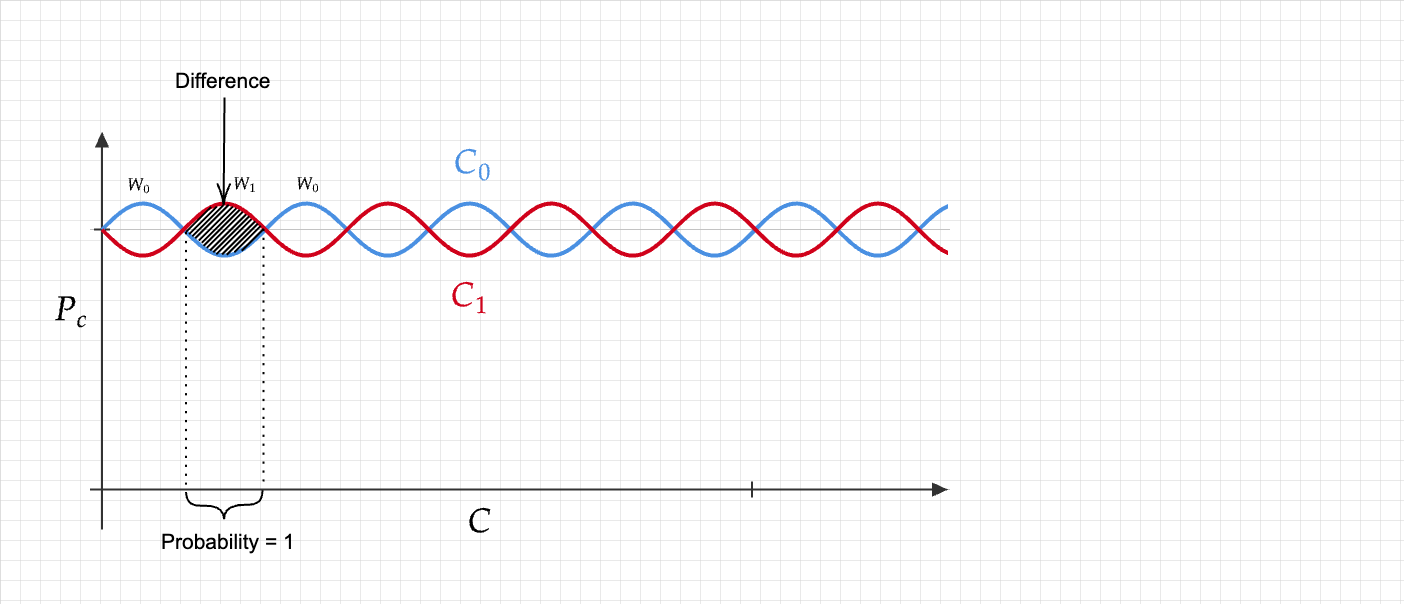
\includegraphics[scale=0.25]{assets/week1-statistical-distance.png}
\end{figure}

If the curve is straight and there is no difference then it is "perfect" hiding. 

$$
\begin{matrix}
    c \in W_0: && \mathbf{Output} \: 0 \\
    c \in W_1: && \mathbf{Output} \: 1 \\
\end{matrix}
$$

Let's define the probabilities as well so we can use them to define \textbf{statistical distance}.

$$
Pr_{r_1} [A(c_1) = 1] = \sum_{c \in W_1} P_r[C \leftarrow c_1]
$$

$$
Pr_{r_0} [A(c_0) = 1] = \sum_{c \in W_1} P_r[C \leftarrow c_0]
$$

We can then say the statistical distance between $c_0$ and $c_1$ is as follows:

$$
SD(c_0, c_1) = \frac{1}{2} \sum_c |P_r[C \leftarrow c_0] - P_r[C \leftarrow c_1]|
$$

Now, let's define small.

\begin{itemize}
    \item If "small" = 0 then it is perfect hiding. The curves are the same.
    \item If "small" = Negligible then it is statistical hiding.
\end{itemize}

\textbf{You cannot have both perfect hiding and binding}

\section{Encryption Based Commitment Schemes}

\subsection{El Gamal}

$$
Gen(1^\lambda) \rightarrow (G,g,h = g^a) = PP
$$

$a$ = secret key.

$$
\mathbf{Commit}_{pp}(b;r) \rightarrow (g^r, h^r \cdot g^b)
$$

It has computational hiding and perfect binding. Under the assumption of DDH is hard.

\subsection{Discrete Log}

Let's define public parameters
\begin{align*}
    Gen(1^\lambda) \rightarrow (G,g,p) \\
    h \leftarrow G \\
    h = g^e, e \in \mathbb Z_p \\
    return (G,g,p,h)
\end{align*}

Let's define other functions $\mathbf{CheckParams}$, $\mathbf{Commit}$:

\begin{align*}
    \mathbf{CheckParams(PP)}: \text{Verify } h \in G, \text{ Check}(G,g,p) \\
    \mathbf{Commit}_{pp}(b;r \in Z_p): return \: c = h^b \cdot g^r
\end{align*}

To prove it is perfect hiding and computational binding let's go over each.

\subsubsection{Proving Perfect Hiding}

Consider commitment $c = g^r \cdot h^b$.

Let's take two $(r_0, r_1)$ such that $b = 0$ or $b = 1$ for each $r$.

For any element $c$ in our group $G$, there exists exactly one choice or randomness $r_0 \in \mathbb Z_p$ such that $g \cdot r_0 = c$ and exactly one choice of randomness $r_1 \in \mathbb Z_q$ such that $h \cdot g^{r_1} = c$. Therefore, each $c$ occurs with the same probability, regardless of the bit committed to, i.e. the distribution of $c$ is independent of the choice of the committed bit $b$.


\subsubsection{Proving Computational Binding}\label{dl-comp-binding-proof}

We will use reduction and contradiction to prove it.

\begin{figure}[h]
    \centering
    

\tikzset{every picture/.style={line width=0.75pt}} %set default line width to 0.75pt        

\begin{tikzpicture}[x=0.75pt,y=0.75pt,yscale=-1,xscale=1]
%uncomment if require: \path (0,300); %set diagram left start at 0, and has height of 300

%Shape: Rectangle [id:dp6384526612545285] 
\draw   (116,23.5) -- (567,23.5) -- (567,268.5) -- (116,268.5) -- cycle ;
%Shape: Square [id:dp025027335054112365] 
\draw   (278.75,83.25) -- (404.25,83.25) -- (404.25,208.75) -- (278.75,208.75) -- cycle ;
%Straight Lines [id:da3372624387913161] 
\draw    (71,146.5) -- (114,146.5) ;
\draw [shift={(116,146.5)}, rotate = 180] [color={rgb, 255:red, 0; green, 0; blue, 0 }  ][line width=0.75]    (10.93,-3.29) .. controls (6.95,-1.4) and (3.31,-0.3) .. (0,0) .. controls (3.31,0.3) and (6.95,1.4) .. (10.93,3.29)   ;
%Straight Lines [id:da2947669535047672] 
\draw  [dash pattern={on 0.84pt off 2.51pt}]  (116,146.5) -- (276,146.5) ;
\draw [shift={(278,146.5)}, rotate = 180] [color={rgb, 255:red, 0; green, 0; blue, 0 }  ][line width=0.75]    (10.93,-3.29) .. controls (6.95,-1.4) and (3.31,-0.3) .. (0,0) .. controls (3.31,0.3) and (6.95,1.4) .. (10.93,3.29)   ;
%Straight Lines [id:da47787602379667105] 
\draw    (405,146.5) -- (442,146.5) ;
\draw [shift={(444,146.5)}, rotate = 180] [color={rgb, 255:red, 0; green, 0; blue, 0 }  ][line width=0.75]    (10.93,-3.29) .. controls (6.95,-1.4) and (3.31,-0.3) .. (0,0) .. controls (3.31,0.3) and (6.95,1.4) .. (10.93,3.29)   ;
%Straight Lines [id:da9499600755580224] 
\draw    (567,143.5) -- (610,143.5) ;
\draw [shift={(612,143.5)}, rotate = 180] [color={rgb, 255:red, 0; green, 0; blue, 0 }  ][line width=0.75]    (10.93,-3.29) .. controls (6.95,-1.4) and (3.31,-0.3) .. (0,0) .. controls (3.31,0.3) and (6.95,1.4) .. (10.93,3.29)   ;

% Text Node
\draw (534,38) node [anchor=north west][inner sep=0.75pt]   [align=left] {$\displaystyle R$};
% Text Node
\draw (379,92) node [anchor=north west][inner sep=0.75pt]   [align=left] {$\displaystyle A$};
% Text Node
\draw (25,117) node [anchor=north west][inner sep=0.75pt]   [align=left] {$\displaystyle ( G,p,g,h)$};
% Text Node
\draw (431,119) node [anchor=north west][inner sep=0.75pt]   [align=left] {$\displaystyle r_{0} ,\ r_{1}$};
% Text Node
\draw (621,135) node [anchor=north west][inner sep=0.75pt]   [align=left] {$\displaystyle e$};
% Text Node
\draw (455,187) node [anchor=north west][inner sep=0.75pt]   [align=left] {$\displaystyle g^{r_{0}} =\ h\cdotp g^{r_{1}}$};
% Text Node
\draw (25,90) node [anchor=north west][inner sep=0.75pt]   [align=left] {$\displaystyle 1$};
% Text Node
\draw (156,120) node [anchor=north west][inner sep=0.75pt]   [align=left] {$\displaystyle 2$};
% Text Node
\draw (418,101) node [anchor=north west][inner sep=0.75pt]   [align=left] {$\displaystyle 3$};
% Text Node
\draw (425,207) node [anchor=north west][inner sep=0.75pt]   [align=left] {$\displaystyle 4$};
% Text Node
\draw (607,117) node [anchor=north west][inner sep=0.75pt]   [align=left] {$\displaystyle 5$};
% Text Node
\draw (572,163) node [anchor=north west][inner sep=0.75pt]   [align=left] {Such that $\displaystyle h\ =\ g^{e}$};
% Text Node
\draw (176,276.5) node [anchor=north west][inner sep=0.75pt]  [font=\scriptsize] [align=left] {Divide expression ($\displaystyle 4$), by $\displaystyle g^{r_{1}}$ on both sides};
% Text Node
\draw (449,270) node [anchor=north west][inner sep=0.75pt]   [align=left] {$\displaystyle g^{r_{0} -r_{1}} =\ h$};
% Text Node
\draw (580,274) node [anchor=north west][inner sep=0.75pt]   [align=left] {$\displaystyle r_{0} \ -\ r_{1}\bmod p$};
% Connection
\draw    (526,282.27) -- (575,282.61) ;
\draw [shift={(577,282.62)}, rotate = 180.39] [color={rgb, 255:red, 0; green, 0; blue, 0 }  ][line width=0.75]    (10.93,-3.29) .. controls (6.95,-1.4) and (3.31,-0.3) .. (0,0) .. controls (3.31,0.3) and (6.95,1.4) .. (10.93,3.29)   ;
% Connection
\draw    (456.78,215) -- (306.9,271.79) ;
\draw [shift={(305.03,272.5)}, rotate = 339.25] [color={rgb, 255:red, 0; green, 0; blue, 0 }  ][line width=0.75]    (10.93,-3.29) .. controls (6.95,-1.4) and (3.31,-0.3) .. (0,0) .. controls (3.31,0.3) and (6.95,1.4) .. (10.93,3.29)   ;
% Connection
\draw    (379,282.76) -- (444,282.3) ;
\draw [shift={(446,282.29)}, rotate = 179.59] [color={rgb, 255:red, 0; green, 0; blue, 0 }  ][line width=0.75]    (10.93,-3.29) .. controls (6.95,-1.4) and (3.31,-0.3) .. (0,0) .. controls (3.31,0.3) and (6.95,1.4) .. (10.93,3.29)   ;

\end{tikzpicture}
\end{figure}

If the discrete log problem is hard in our group, then given an element $h$ in our group, it should be hard to find the exponent $e$ such that $g^e = h$. We can build a reduction $R$ that uses any adversary $A$ that breaks binding to solve for the discrete log of $h$. Given the discrete log challenge $(G, p, g, h)$, $R$ gives $pp = (G, p, g, h)$ to $A$. $A$ then comes up with $r_0, r_1$ such that
$$\mathbf{Commit}_{pp}(0; r_0) = \mathbf{Commit}_{pp}(1; r_1)$$
that is, $g^{r_0} =h \cdot g^{r_1}$. $R$ can then solve for the discrete log of $h$ by setting $e=r_0−r_1 (\mod p)$.

\pagebreak

\hrule
\hrule
\vspace{0.2cm}
\begin{center}
    February 2, 2024 (TA Session)
\end{center}
\vspace{0.3cm}
\hrule
\hrule
\begin{center}
    \textsc{Week 1 - Other Commitment Schemes}
\end{center}

\section{Recap}

Commitments $\neq$ Encryption. There are difference in between them.

In commitment, there is no $\mathbf{Decryption}$ function but it does provide $\mathbf{Binding}$. You can consider encrypt with perfect correctness $\rightarrow$ commit.

\subsection{Binding Advantage}\label{binding-advantage}
$$
P_r[A(pp) \rightarrow (r_0, r_1) | \mathbf{Commit}_{pp}(0;r_0) = \mathbf{Commit}_{pp}(1;r_1)] = Small
$$
\subsection{Hiding Advantage}\label{hiding-advantage}
$$
Pr_{r_0} [A(\mathbf{Commit}_{pp}(0;r_0))) = 1] - Pr_{r_1} [A(\mathbf{Commit}_{pp}(1;r_1)) = 1] = Small
$$

\subsection{Commitment Properties Overview}


\begin{table}[h]
\begin{tabular}{|l|l|l|l|l|l|}
\hline
\multicolumn{1}{|c|}{\textbf{Property}} &
  \multicolumn{1}{c|}{\textbf{Description}} &
  \multicolumn{1}{c|}{\textbf{Advantage}} &
  \multicolumn{1}{c|}{\textbf{Type}} &
  \textbf{Sub-Type} &
  \textbf{Small Definition} \\ \hline
\multirow{2}{*}{Binding} &
  \multirow{2}{*}{For any $A$} &
  \multirow{2}{*}{Binding Advantage (\ref{binding-advantage})} &
  Computational &
  - &
  Negligible \\ \cline{4-6} 
 &
   &
   &
  Unconditional or Perfect &
  - &
  Impossible \\ \hline
\multirow{3}{*}{Hiding} &
  \multirow{3}{*}{For any $A$} &
  \multirow{3}{*}{Hiding Advantage (\ref{hiding-advantage})} &
  Computational &
  - &
  Negligible \\ \cline{4-6} 
 &
   &
   &
  \multirow{2}{*}{Unconditional*} &
  Statistical &
  Negligible \\ \cline{5-6} 
 &
   &
   &
   &
  Perfect &
  Impossible \\ \hline
\end{tabular}
\end{table}

* Notice that for hiding the unconditional is not directly perfect like binding. It actually has two sub-types.


\section{Encryption Based Schemes (Cont.)}

\begin{table}[h]
\begin{tabular}{|l|l|l|l|l|}
\hline
\multicolumn{1}{|c|}{\textbf{Construction}} &
  \multicolumn{1}{c|}{\textbf{Binding}} &
  \multicolumn{1}{c|}{\textbf{Hiding}} &
  \multicolumn{1}{c|}{\textbf{Assumption}} &
  \multicolumn{1}{c|}{\textbf{Param Generation Ownership}} \\ \hline
El Gamal                             & Perfect       & Computational & DDH is Hard                        & Prover (P) \\ \hline
Discrete Log                         & Computational & Perfect       & Discrete Log is Hard               & Verifier (V) \\ \hline
hOWF & Computational & Perfect       & hOWF is Hard                       & Verifier (V) \\ \hline
{[}Haitner, Reingold{]}              & Computational & Statistical   & OWF is Hard                        &              \\ \hline
{[}Naor{]}                           & Perfect       & Computational & OWF = PRG &              \\ \hline
{[}Naor-Yung{]}                      & Computational & Statistical   & CRH &              \\ \hline
\end{tabular}
\end{table}

*hOWF = Homomorphic One-Way Functions \\
**PRG = Pseudorandom Generator \\
***CRH = Collision Resistance Hashing

\subsection{El Gamal}

In the ElGamal commitment scheme, the prover generates the public parameters to ensure the integrity and security of the commitment. The public parameters are generated as follows:

$$
Gen(1^\lambda) \rightarrow (G,g,h = g^a) = PP
$$

Here, $a$ is the prover's secret key, $G$ is a multiplicative group, $g$ is a generator of $G$, and $h$ is the public key.

If the verifier were to generate the public parameters, they could potentially exploit the system in several ways:

\begin{itemize}
    \item \textbf{Knowledge of the secret key}: If the verifier generates the public key, they would know the corresponding secret key $a$. This could allow them to decrypt any message or commitment, violating the confidentiality of the commitment scheme.
    \item \textbf{Non-binding commitments}: If the verifier knows the secret key $a$, they could manipulate the commitment. For instance, for a given commitment
\end{itemize}

$$
\mathbf{Commit}_{pp}(b;r) \rightarrow (g^r, h^r \cdot g^b)
$$

(where $b$ is the message and $r$ is a random number), the verifier could choose a different message $b'$ and solve for $r'$ in the equation $b + ar \cong b' + ar' (mod \: q)$. This would allow the commitment to be opened to different values $(b', r')$, making the commitment non-binding.

Therefore, to maintain the security properties of the ElGamal commitment scheme, it's crucial that the prover generates the public parameters.

\subsection{Discrete Log}

In a discrete logarithm-based commitment scheme, the verifier generates the parameters to ensure the integrity and security of the commitment. If the prover does it then

\textbf{Non-binding commitments}: If the prover knows the secret key $e$, they could manipulate the commitment. For instance, for a given commitment 

\[
\mathbf{Commit}_{pp}(b;r) \rightarrow c = h^b \cdot g^r
\]

(where $b$ is the message and $r$ is a random number), the prover could choose a different message $b'$ and solve for $r'$ in the equation $b + er \cong b' + er' (mod \: p)$. This would allow the prover to fool the verifier by using a different values $(b', r')$ which satisfy the discrete log , making the commitment non-binding.


\subsection{Homomorphic One-Way Functions (DL)}

Let's define the commitment scheme between the prover and verifier that uses function $f(x) = g^x$ since it is based on DL:

$\mathbf{Gen}(1^{\lambda})$: Choose $f$; choose $h$ in the image of $f$. Let $PP = (f,h)$.

$\mathbf{CheckParams}(pp)$: Check that $f$ is a one-way homomorphism of the expected form, and that $h$ is in the image of $f$.

\begin{align*}
    c = \mathbf{Commit}_{pp}(b,r) \\
    = f(r), \text{ if } b = 0 \\
    = h \cdot f(r), \text{ if } b = 1
\end{align*}


\subsubsection{Homomorphism}
There are certain requirements for the $f$ function to be homomorphic. Which are as follows:

\begin{enumerate}
    \item $f$ must be one-way - meaning, there shouldn't be any pre-image of it. It should be hard to find $x$ if you are give $g^x$
    \item It needs homomorphism - meaning, $f(a) + f(b) = f(a+b)$
    \item If a function $f$ is multiplied by any value $h$ as mentioned above. This should result into a permutation.
\end{enumerate}

\subsubsection{Proving Computational Binding}

Refer section \ref{dl-comp-binding-proof}

\subsubsection{Proving Perfect Hiding}

\textbf{Goal}: Find the inverse of $f$ such that we can break the hOWF assumption.

\begin{figure}[h]
    \centering
    

\tikzset{every picture/.style={line width=0.75pt}} %set default line width to 0.75pt        

\begin{tikzpicture}[x=0.75pt,y=0.75pt,yscale=-1,xscale=1]
%uncomment if require: \path (0,300); %set diagram left start at 0, and has height of 300

%Shape: Rectangle [id:dp250033178836363] 
\draw   (100,22.5) -- (551,22.5) -- (551,267.5) -- (100,267.5) -- cycle ;
%Shape: Square [id:dp5707708728044976] 
\draw   (262.75,82.25) -- (388.25,82.25) -- (388.25,207.75) -- (262.75,207.75) -- cycle ;
%Straight Lines [id:da6813221557375704] 
\draw    (55,145.5) -- (98,145.5) ;
\draw [shift={(100,145.5)}, rotate = 180] [color={rgb, 255:red, 0; green, 0; blue, 0 }  ][line width=0.75]    (10.93,-3.29) .. controls (6.95,-1.4) and (3.31,-0.3) .. (0,0) .. controls (3.31,0.3) and (6.95,1.4) .. (10.93,3.29)   ;
%Straight Lines [id:da4601588592518926] 
\draw  [dash pattern={on 0.84pt off 2.51pt}]  (100,145.5) -- (260,145.5) ;
\draw [shift={(262,145.5)}, rotate = 180] [color={rgb, 255:red, 0; green, 0; blue, 0 }  ][line width=0.75]    (10.93,-3.29) .. controls (6.95,-1.4) and (3.31,-0.3) .. (0,0) .. controls (3.31,0.3) and (6.95,1.4) .. (10.93,3.29)   ;
%Straight Lines [id:da6326313588425969] 
\draw    (389,145.5) -- (426,145.5) ;
\draw [shift={(428,145.5)}, rotate = 180] [color={rgb, 255:red, 0; green, 0; blue, 0 }  ][line width=0.75]    (10.93,-3.29) .. controls (6.95,-1.4) and (3.31,-0.3) .. (0,0) .. controls (3.31,0.3) and (6.95,1.4) .. (10.93,3.29)   ;
%Straight Lines [id:da019622542541199106] 
\draw    (551,142.5) -- (594,142.5) ;
\draw [shift={(596,142.5)}, rotate = 180] [color={rgb, 255:red, 0; green, 0; blue, 0 }  ][line width=0.75]    (10.93,-3.29) .. controls (6.95,-1.4) and (3.31,-0.3) .. (0,0) .. controls (3.31,0.3) and (6.95,1.4) .. (10.93,3.29)   ;

% Text Node
\draw (518,37) node [anchor=north west][inner sep=0.75pt]   [align=left] {$\displaystyle R$};
% Text Node
\draw (363,91) node [anchor=north west][inner sep=0.75pt]   [align=left] {$\displaystyle A$};
% Text Node
\draw (9,116) node [anchor=north west][inner sep=0.75pt]   [align=left] {$\displaystyle ( f,h)$};
% Text Node
\draw (415,118) node [anchor=north west][inner sep=0.75pt]   [align=left] {$\displaystyle r_{0} ,\ r_{1}$};
% Text Node
\draw (604,134) node [anchor=north west][inner sep=0.75pt]   [align=left] {$\displaystyle e\ =\ r_{0} -r_{1}$};
% Text Node
\draw (418,166) node [anchor=north west][inner sep=0.75pt]   [align=left] {$\displaystyle f( r_{0}) \ =\ h\ \cdotp f( r_{1})$};
% Text Node
\draw (9,89) node [anchor=north west][inner sep=0.75pt]   [align=left] {$\displaystyle 1$};
% Text Node
\draw (140,119) node [anchor=north west][inner sep=0.75pt]   [align=left] {$\displaystyle 2$};
% Text Node
\draw (402,100) node [anchor=north west][inner sep=0.75pt]   [align=left] {$\displaystyle 3$};
% Text Node
\draw (339,216) node [anchor=north west][inner sep=0.75pt]   [align=left] {$\displaystyle 4$};
% Text Node
\draw (591,116) node [anchor=north west][inner sep=0.75pt]   [align=left] {$\displaystyle 5$};
% Text Node
\draw (556,162) node [anchor=north west][inner sep=0.75pt]   [align=left] {Such that $\displaystyle f( e) =h$};
% Text Node
\draw (123,276.5) node [anchor=north west][inner sep=0.75pt]  [font=\scriptsize] [align=left] {Divide expression ($\displaystyle 4$), by $\displaystyle f( r_{1})$ on both sides};
% Text Node
\draw (433,269) node [anchor=north west][inner sep=0.75pt]   [align=left] {$\displaystyle f( r_{0} -r_{1}) =\ h$};
% Text Node
\draw (571,268) node [anchor=north west][inner sep=0.75pt]   [align=left] {$\displaystyle r_{0} \ -\ r_{1}\bmod p$};
% Connection
\draw    (538,277.61) -- (566,277.41) ;
\draw [shift={(568,277.4)}, rotate = 179.59] [color={rgb, 255:red, 0; green, 0; blue, 0 }  ][line width=0.75]    (10.93,-3.29) .. controls (6.95,-1.4) and (3.31,-0.3) .. (0,0) .. controls (3.31,0.3) and (6.95,1.4) .. (10.93,3.29)   ;
% Connection
\draw    (449.97,188) -- (253.33,271.72) ;
\draw [shift={(251.49,272.5)}, rotate = 336.94] [color={rgb, 255:red, 0; green, 0; blue, 0 }  ][line width=0.75]    (10.93,-3.29) .. controls (6.95,-1.4) and (3.31,-0.3) .. (0,0) .. controls (3.31,0.3) and (6.95,1.4) .. (10.93,3.29)   ;
% Connection
\draw    (336,280.6) -- (428,278.98) ;
\draw [shift={(430,278.95)}, rotate = 178.99] [color={rgb, 255:red, 0; green, 0; blue, 0 }  ][line width=0.75]    (10.93,-3.29) .. controls (6.95,-1.4) and (3.31,-0.3) .. (0,0) .. controls (3.31,0.3) and (6.95,1.4) .. (10.93,3.29)   ;

\end{tikzpicture}

\end{figure}

In the book instead of $f(a+b) = f(a) + f(b)$ as show above, it uses $f(a \cdot b) = f(a) \cdot f(b)$. So, the reduction will be updated accordingly.

\subsection{Haitner, Reingold}

Not discussed.

\subsection{Recap: PRG}

A pseduorandom generator $G$ takes a smaller input space and maps to a bigger output space which is truly random.

$$
G:\{0,1\}^{\lambda} \rightarrow \{0,1\}^{3\cdot \lambda}
$$

For all PPT $A$, such that

\begin{itemize}
    \item Pseudorandom Generator (PRG): A PRG is a deterministic procedure that takes a truly random seed and stretches it into a longer pseudorandom string. The function $G$ takes an input string of length $\lambda$ and outputs a string of length $3\cdot \lambda$.
    \item Probabilistic Polynomial Time (PPT): $A$ is a PPT algorithm. This means that $A$ is a randomized algorithm that runs in polynomial time in the length of its input.
    \item Negligible Function: A function $f$ is negligible if for every positive polynomial $p$ and all sufficiently large $n$, $f(n) < 1/p(n)$. In other words, $f(n)$ becomes insignificantly small as $n$ grows.
\end{itemize}


$$
P_r[A(G(r)) = 1] - P_r[A(r) = 1] = negligible
$$

It states that for all PPT algorithms $A$, the probability that $A$ can distinguish the output of the PRG $G(r)$ from a truly random string $r$ is negligible. 

\subsection{Naor}

This uses PRG (fixed $G, h$) such that the public parameters looks as follows:

$$PP = G, h \in \{0,1\}^{3 \cdot \lambda}$$

Let's define the commitment between prover and verifier as follows:

\begin{align*}
    c = \mathbf{Commit}_{pp}(b \in \{0,1\}^{\lambda}, r \in \{0,1\}^{\lambda}) \\
    \begin{matrix}
        = G(r) \oplus h, && \text{ If } b = 1 \\
        = G(r), && \text{ If } b = 0 \\
    \end{matrix}
\end{align*}

\subsubsection{Proving Perfect Binding}

To prove this we have to break it such that we find pair $(r_0, r_1)$ that commits to same thing so $$G(r_0) = G(r_1) \oplus h$$.

If we have $(r_0, r_1)$, then we have $2^{\lambda^{2}}$  because each $r$ has $2^\lambda$. So, overall we have $2^{2\lambda}$ choices. Then there are only these many possible valid offsets $\delta$ such that $G(r_0) \oplus G(r_1) = \delta$ that there could exist a collision.

We are picking $h$ from $3 \dot \lambda$ space, so there are $2^{3\cdot \lambda}$ choices.

So, the probability that h is a valid offset is -

$$
P_r[\text{h is a valid offset}] = \frac{2^{2\lambda}}{2^{3\lambda}} = 2^{-\lambda} 
$$

This is very small, negligible. The argument for unconditional binding, we want this small to be $0$. So, if we pick $h$ at random, and its a good $h$ which is possible with overwhelming possibility since we have $3\lambda$ space to pick from. So, it is truly random.

The public parameters are picked by prover.

\subsubsection{Proving Computational Hiding}

We need to prove the following:

$$C_0 \thicksim_c U \thicksim_c C_1$$

This above statement means that there is a distribution of commitment with 0 that is computationally indistinguishable from a uniform random distribution that is computationally indistinguishable to the distribution of commitment with 1.

This implies that $C_0 \thicksim_c C_1$. [Proved in exercise 2 in commitment book]

We will prove it using reduction. We are using PRG, we want our reduction $R$ to take in either a truly uniformly random string ($U_{3\lambda}$) or a $G(U_{\lambda})$. It takes a sample from one of these and it makes a guess if it is random or a result from PRG.

\textbf{Proving $C_0 \thicksim_c U$}

We take this adversary $A$, that takes $C_0$ and $U_{3\lambda}$ which can discerns between the distributions. $C_0$ = PRG applied to a random value. A sample from G(r) is really just a sample from commitments to $0$. If $A$ has some non negligible advantage that can discern in between them. then the reduction has the non negligible advantage to distinguish between them too.

\textbf{Proving $U \thicksim_c C_1$}

An oracle gives us an $h$ and we $\oplus$ it with a uniform value. If the adversary can tell the difference between the $h \oplus$ on a random bit results a random permutation and the value generated from $3\lambda$ space. Then we can say $R$ also has the non negligible advantage. Therefore, we can say there is a computational hiding.

\subsection{Naor-Yung}

This uses the concept of CRH (collision resistant hashing). Which means that it is hard to find a function ($H$) that has a collision.

$$
H(x_0) = H(x_1) | x_0 \neq x_1
$$

There is always a collision in hash functions because the function $H$ maps a fixed space to a smaller space which holds because of the pigeon-hole principle.

Public Parameters are defined as follows:

$$
H:\{0,1\}^{2\cdot \lambda} \rightarrow \{0,1\}; PP = H
$$

We then define the commitment as follows:

$$
C = \mathbf{Commit}_{pp}(b; (r \in \{0,1\}^{2\cdot \lambda}, x \in \{0,1\}^{2\cdot \lambda})) \\
= (h(x), r, (r \cdot x) \oplus b)
$$

\subsubsection{Proving Computational Binding}

We will do it by reduction, where our goal is to find $H$ where we do have a collision. Our reduction $R$ will break the collision resistance, therefore it will take an $H$ and produce $x_0, x_1$ such that $H(x_0) = H(x_1)$ but $x_0 \neq x_1$. We take an adversary $A$ that breaks computational binding.

We give this adversary $A$, the $H$ hash function. It produces two pairs $r_0, x_0$ and $r_1, x_1$ such that -

\begin{align*}
    c_0 = (h(x_0), r_0, (r_0 \cdot x_0) \oplus 0) \\
    \Rightarrow (h(x_0), r_0, (r_0 \cdot x_0)) \\
    c_1 = (h(x_1), r_1, (r_1 \cdot x_1) \oplus 1)
\end{align*}

Since, $r$ appears entirely in the commitment then it means that $r_0 = r_1$ which is non-negotiable. We also know that $H(x_0) = H(x_1)$ under assumption. What about $r_0 \cdot x_0 = r_1 \cdot x_1$? No. Then if $r_0 \cdot x_0 \neq r_1 \cdot x_1$ then $x_0 \neq x_1$ which means that there is a collision.


\textbf{"Since, $r$ appears entirely in the commitment then it means that $r_0 = r_1$?"}: This statement is referring to the fact that the same random value $r$ is used in both commitments $c_0$ and $c_1$. In the Naor-Yung scheme, the same $r$ value is used to create both commitments. Therefore, if an adversary is able to produce two valid commitments, they must have used the same $r$ value in both, hence $r_0 = r_1$.

\textbf{"What about $r_0 \cdot x_0 = r_1 \cdot x_1$? No"} This statement is saying that even though $r_0 = r_1$, it does not necessarily mean that $r_0 \cdot x_0 = r_1 \cdot x_1$. This is because $x_0$ and $x_1$ are different values (as per the assumption that $H(x_0) = H(x_1)$ but $x_0 \neq x_1$). Therefore, even if the same $r$ value is used, the results of $r_0 \cdot x_0$ and $r_1 \cdot x_1$ would be different unless $x_0 = x_1$, which contradicts our assumption. Hence, $r_0 \cdot x_0 \neq r_1 \cdot x_1$.
   
\subsubsection{Proving Statistical Hiding}

Check commitment notes.

% \bibliographystyle{unsrtnat}
% \bibliography{references}

\end{document}
